\documentclass[conference]{IEEEtran}
\IEEEoverridecommandlockouts
% The preceding line is only needed to identify funding in the first footnote. If that is unneeded, please comment it out.
\usepackage{cite}
\usepackage{amsmath,amssymb,amsfonts}
\usepackage{algorithmic}
\usepackage{graphicx}
\usepackage{textcomp}
\usepackage{xcolor}
\def\BibTeX{{\rm B\kern-.05em{\sc i\kern-.025em b}\kern-.08em
    T\kern-.1667em\lower.7ex\hbox{E}\kern-.125emX}}
\begin{document}

\title{Edge computing testbed for V2I applications prototyping and evaluation *\\
{\footnotesize \textsuperscript{*}Note: Sub-titles are not captured in Xplore and
should not be used}
\thanks{funded by AT}
}

\author{\IEEEauthorblockN{1\textsuperscript{st} Zeinab Nezami}
\IEEEauthorblockA{\textit{School of Computing} \\
\textit{University of Leeds}\\
Leeds, United Kingdom \\
email address or ORCID}
\and
\IEEEauthorblockN{2\textsuperscript{nd} Evangelos Pournaras}
\IEEEauthorblockA{\textit{School of Computing} \\
\textit{University of Leeds}\\
Leeds, United Kingdom \\
email address or ORCID}
\and
\IEEEauthorblockN{6\textsuperscript{th} Given Name Surname}
\IEEEauthorblockA{\textit{dept. name of organization (of Aff.)} \\
\textit{name of organization (of Aff.)}\\
City, Country \\
email address or ORCID}
}

\maketitle

\begin{abstract}

\end{abstract}

\begin{IEEEkeywords}
Edge Computing, V2I application, Testbed, , 
\end{IEEEkeywords}

\section{Introduction}

Challenges: 
ITS applications should deal with various data provided
through various communication links. The density and the
mobility of the vehicles are the major factors to take into account
when developing V2X applications that are destined to run in
mobile edge computing distributed environment. In a high-density
scenario, the application must use the available bandwidth
efficiently in order to deliver its service continuously to the
subscribed nodes. The application should also deal with nodes
joining/leaving the network during their mouvement and
guarantee the service continuity. The MEC infrastructure is
intended to offer a management system and a couple of standard
services that facilitate the aforementioned properties. The MEC
infrastructure introduces a whole new service model that requires
an adapted development paradigm.
An important aspect that should be taken into account while
developing a V2X application that targets MEC as a deployment
environment is to ensure the proper interaction of the application
with the management entities and the system components. At the
development phase of a V2X MEC service components testing in
real environment increase deployment time, costs, and
complexity. In the next section, we analyze the standard
deployment architecture proposed by the European
Telecommunications Standards Institute (ETSI) to extract the
main components and their functionalities.

\section{Related work}
\begin{table}[htbp]
\caption{Table Type Styles}
\begin{center}
\begin{tabular}{|c|c|c|c|}
\hline
\textbf{Table}&\multicolumn{3}{|c|}{\textbf{Table Column Head}} \\
\cline{2-4} 
\textbf{Head} & \textbf{\textit{Table column subhead}}& \textbf{\textit{Subhead}}& \textbf{\textit{Subhead}} \\
\hline
copy& More table copy$^{\mathrm{a}}$& &  \\
\hline
\multicolumn{4}{l}{$^{\mathrm{a}}$Sample of a Table footnote.}
\end{tabular}
\label{tab1}
\end{center}
\end{table}

\begin{figure}[htbp]
\centerline{
\includegraphics{fig1.png}}
\caption{Example of a figure caption.}
\label{fig}
\end{figure}
\section{Testbed Design}
\par The proposed testbed aims at helping researchers and developers to design and verify distributed
V2I applications and algorithms destined to run in an edge computing environment. 

The main components of the testbed includes agent, network infrastructure, service distributor, connector, and system orchestrator.
\par As shown in fig\ref{fig-arch} the testbed is modelled using the modules presented as follows.

\subsection{agent}
\par An agent is an abstraction of a mobile entity such as vehicle or mobile device equipped with a set of sensors (e.g., GPS, camera), enabling the surrounding environment perception (e.g., position, speed, temperature) and a set of actuators (e.g., display, acceleration). 

\subsubsection{Mobility support}
Each user has a mobility profile 

In order to initiate/update vehicle nodes position, create/destroy communication's virtual links, and manage mobility
models a mobility API is developed. 
\par The developed mobility API can be used to implement different mobility models. 
A real-world map, in our tests Munich city map, could be imported to the SUMO mobility simulator to model an accurate mobility model that simulates vehicle movements. 
The nodes positions could be extracted through the interaction with a real-world map offered by the interconnection with a mobility model that calculates the successive node position following the implemented mobility model. 
The mobility support is achieved through the use of the mobile nodes’ positions regarding the fixed edge nodes and the city map to create and destroy communication links in runtime.

\subsubsection{Network infrastructure}
\par\emph {Edge nodes}: the edge infrastructure offers a distributed limited storage and processing capabilities in the vicinity of the agents to cope with the Cloud issues regarding real-time services ultra-low latency requirements.
 Edge computing offers ultra-low latency, high bandwidth, and real-time access to radio network information that can be leveraged by an emerging vehicular safety and navigating applications. The "edge node" term refers to the combination of base stations (or access points) and edge servers close to the mobile radio network. 
 
 Each edge node has a fixed position in a city that is the input provided by the developer.

\par\emph {Cloud center}: the Cloud offers a centralized high storage and processing capabilities to collect and process massive data volumes to provide customized ITS services to different vehicles.
\par\emph {Connector} :cellular networks are characterized by a wide communication range, which allows a base station to maintain connectivity with a network node (vehicle) as long as possible, which means fewer handover operations. The upcoming Fifth Generation cellular network (5G) is one of the leading technologies that promises to grant a very high network capacity that guarantees high throughput/bandwidth for demanding applications. According to [13], 5G networks will natively include mobile edge computing capabilities by design that may support different vehicular communication
technologies. In our testbed, messaging systems like MQTT is responsible for connecting different entities together and synchronising data pipelines. The communication of vehicles with a serving entity through a network is also managed with the connector.

pie and mqtt

\subsection{system orchestrator}
MEC system-level management layer.
The MEO maintains an overall view on available computing,
storage, and networking resources and services. The MEO handles
the task of the appropriate ME host selection for requested
services deployment by taking into account the application
requirements, the available resources, and the nodes' positions.
Finally, The MEO is also responsible for scaling up and down the
available resources as required by the running applications.
Virtualization Infrastructure Manager: Virtualization
Infrastructure Manager (VIM) obviously responsible for
virtualized resources management. The VIM tasks consist of
allocating and releasing the storage, networking, and compute
resources offered by the virtualized infrastructure. VIM could also
store application images for faster instantiation procedure when it
is required. VIM also provides support for fault and performance
monitoring by collecting virtual resources and running application
data and transmitting them to the system level management
entities.
\subsection{Service distributor}




\begin{figure}[htbp]
\centerline{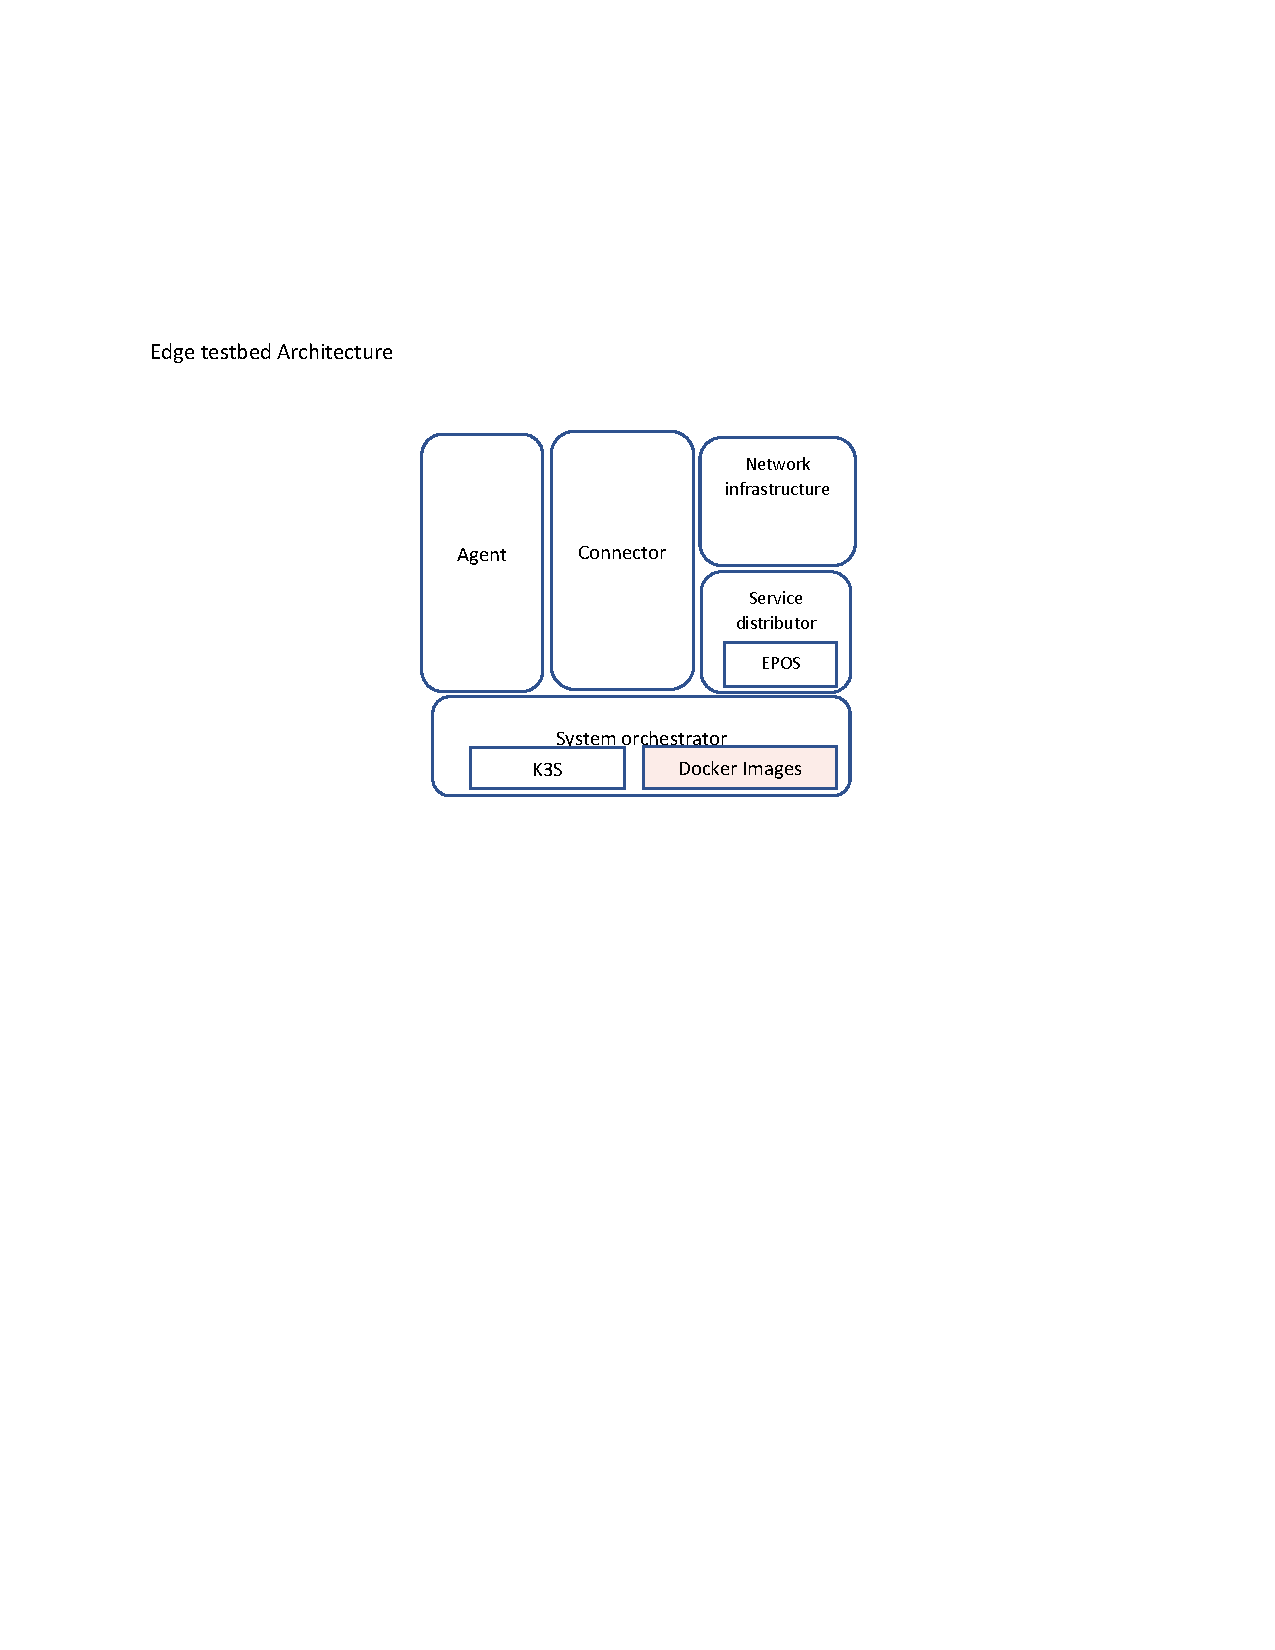
\includegraphics{figures/Arch.pdf}}
\caption{Architecture of proposed test-bed}
\label{fig-arch}
\end{figure}

\subsection{Methodology/ for evaluation}


\section{evaluation}


\subsection{Application/scenario}\label{AA}

\subsection{Threats to validity}


\subsection{Conclusion}

\section*{References}


\end{document}
